\documentclass{article}\usepackage[]{graphicx}\usepackage[]{color}
% maxwidth is the original width if it is less than linewidth
% otherwise use linewidth (to make sure the graphics do not exceed the margin)
\makeatletter
\def\maxwidth{ %
  \ifdim\Gin@nat@width>\linewidth
    \linewidth
  \else
    \Gin@nat@width
  \fi
}
\makeatother

\definecolor{fgcolor}{rgb}{0.345, 0.345, 0.345}
\newcommand{\hlnum}[1]{\textcolor[rgb]{0.686,0.059,0.569}{#1}}%
\newcommand{\hlstr}[1]{\textcolor[rgb]{0.192,0.494,0.8}{#1}}%
\newcommand{\hlcom}[1]{\textcolor[rgb]{0.678,0.584,0.686}{\textit{#1}}}%
\newcommand{\hlopt}[1]{\textcolor[rgb]{0,0,0}{#1}}%
\newcommand{\hlstd}[1]{\textcolor[rgb]{0.345,0.345,0.345}{#1}}%
\newcommand{\hlkwa}[1]{\textcolor[rgb]{0.161,0.373,0.58}{\textbf{#1}}}%
\newcommand{\hlkwb}[1]{\textcolor[rgb]{0.69,0.353,0.396}{#1}}%
\newcommand{\hlkwc}[1]{\textcolor[rgb]{0.333,0.667,0.333}{#1}}%
\newcommand{\hlkwd}[1]{\textcolor[rgb]{0.737,0.353,0.396}{\textbf{#1}}}%
\let\hlipl\hlkwb

\usepackage{framed}
\makeatletter
\newenvironment{kframe}{%
 \def\at@end@of@kframe{}%
 \ifinner\ifhmode%
  \def\at@end@of@kframe{\end{minipage}}%
  \begin{minipage}{\columnwidth}%
 \fi\fi%
 \def\FrameCommand##1{\hskip\@totalleftmargin \hskip-\fboxsep
 \colorbox{shadecolor}{##1}\hskip-\fboxsep
     % There is no \\@totalrightmargin, so:
     \hskip-\linewidth \hskip-\@totalleftmargin \hskip\columnwidth}%
 \MakeFramed {\advance\hsize-\width
   \@totalleftmargin\z@ \linewidth\hsize
   \@setminipage}}%
 {\par\unskip\endMakeFramed%
 \at@end@of@kframe}
\makeatother

\definecolor{shadecolor}{rgb}{.97, .97, .97}
\definecolor{messagecolor}{rgb}{0, 0, 0}
\definecolor{warningcolor}{rgb}{1, 0, 1}
\definecolor{errorcolor}{rgb}{1, 0, 0}
\newenvironment{knitrout}{}{} % an empty environment to be redefined in TeX

\usepackage{alltt}
\usepackage[hmargin = 1in]{geometry}
\usepackage{enumitem}
\usepackage{amsmath, amsthm, amssymb, amsfonts}
\usepackage{booktabs}
\usepackage{tabularx}
\setlist[2]{
font = \color{black},
before = {\color{red}}
}
\setlist[1]{
leftmargin = 0em
}
\usepackage{textcomp}
\IfFileExists{upquote.sty}{\usepackage{upquote}}{}
\begin{document}





\begin{center} \LARGE
Homework 5
\end{center}
\begin{center} \Large
Due February 20, 2020 at 11:59 PM 
\end{center}



\begin{enumerate}
	\item P. 243: 1 
	\begin{enumerate}
	\item (3 points)
	
\begin{knitrout}
\definecolor{shadecolor}{rgb}{0.969, 0.969, 0.969}\color{fgcolor}

{\centering 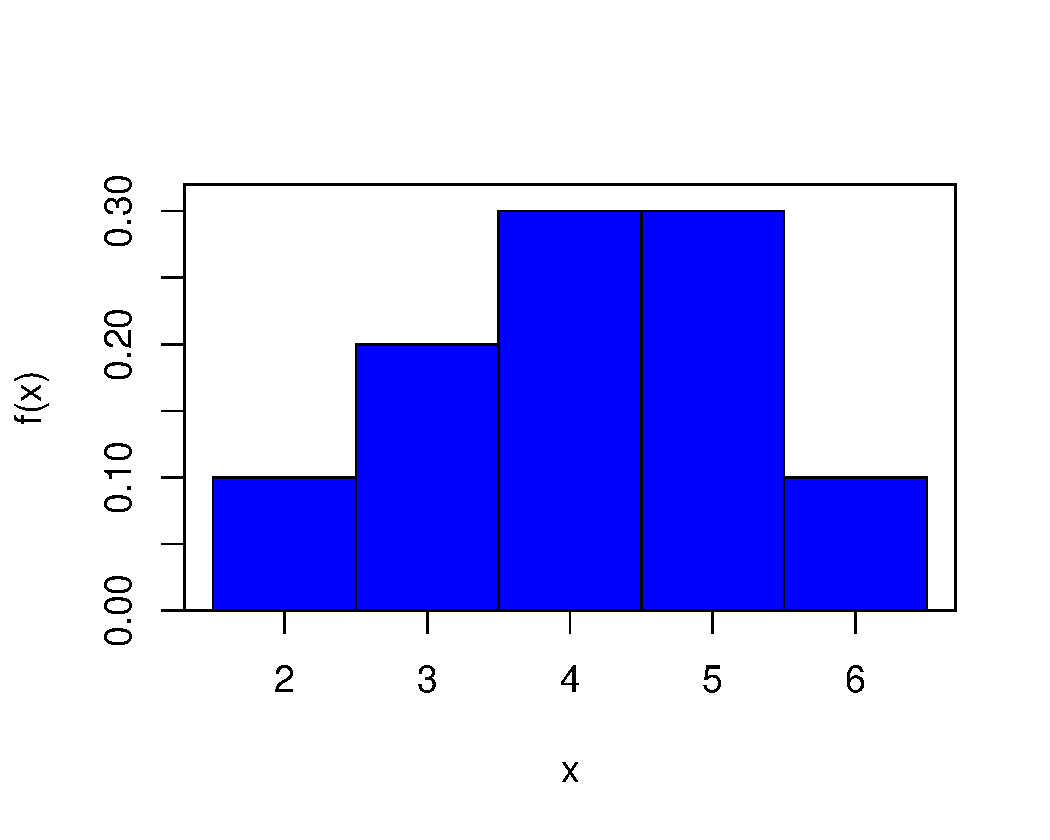
\includegraphics[width=0.6\textwidth]{figure/unnamed-chunk-2-1} 

}




{\centering 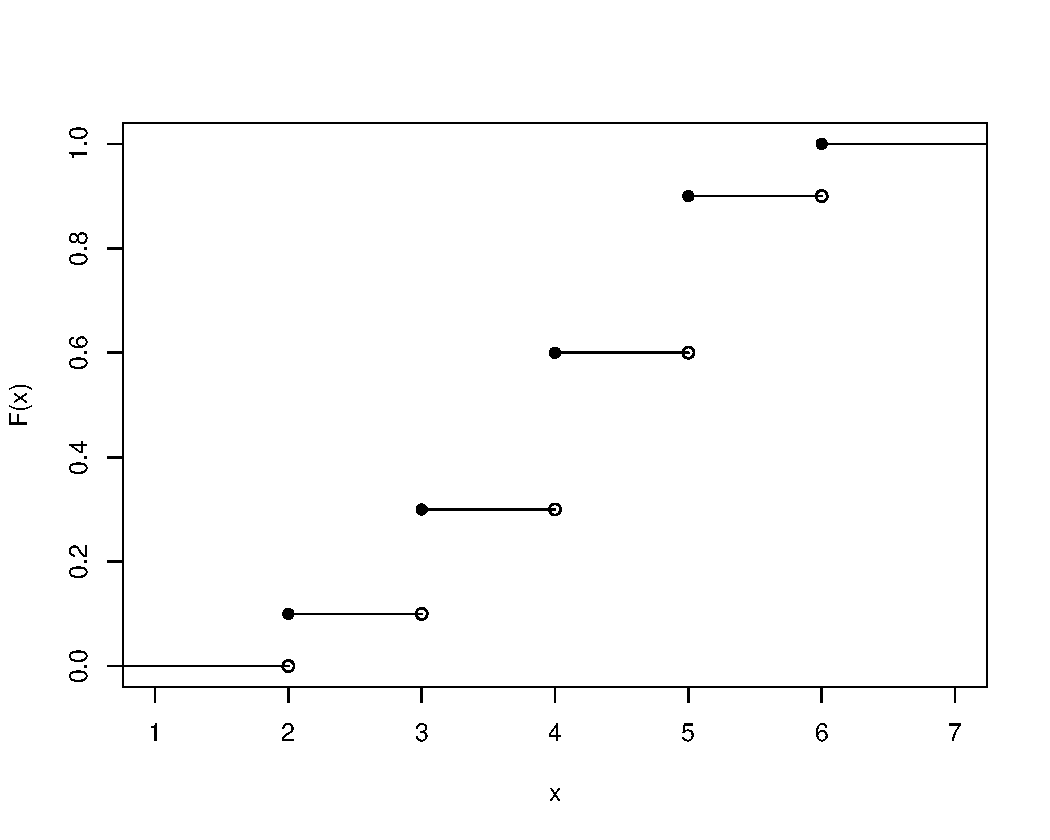
\includegraphics[width=0.6\textwidth]{figure/unnamed-chunk-2-2} 

}



\end{knitrout}


\clearpage
\item (2 points)

$E(X) = 2 (0.1) + 3(0.2) + 4(0.3) + 5(0.4) + 6(0.1) = 4.1$

$E(X^2) = 2^2 (0.1) + 3^2 (0.2) + 4^2 (0.3) + 5^2(0.3) + 6^2 (0.1) = 18.1$, so 
\[Var(X) = E(X^2) - (E(X))^2 = 18.1 - 4.1^2 = 1.29.\]
The standard deviation of $X$ is $\sqrt{1.29} = 1.136$.

  \end{enumerate}
  \clearpage

\item P. 244: 4

{\color{red} (3 points for each $p$)

Use equation (5-3) with $n = 5$.

\begin{knitrout}
\definecolor{shadecolor}{rgb}{0.969, 0.969, 0.969}\color{fgcolor}
\begin{tabular}{>{}r|rrrrrrrrr}
\toprule
$p$ & $f(0)$ & $f(1)$ & $f(2)$ & $f(3)$ & $f(4)$ & $f(5)$ & $E(X) = np$ & $Var(X) = np(1-p)$ & Std.Dev.\\
\midrule
0.1 & 0.5905 & 0.3280 & 0.0729 & 0.0081 & 0.0005 & 0.0000 & 0.5 & 0.45 & 0.671\\
0.3 & 0.1681 & 0.3601 & 0.3087 & 0.1323 & 0.0284 & 0.0024 & 1.5 & 1.05 & 1.025\\
0.5 & 0.0312 & 0.1562 & 0.3125 & 0.3125 & 0.1562 & 0.0312 & 2.5 & 1.25 & 1.118\\
0.7 & 0.0024 & 0.0284 & 0.1323 & 0.3087 & 0.3601 & 0.1681 & 3.5 & 1.05 & 1.025\\
0.9 & 0.0000 & 0.0004 & 0.0081 & 0.0729 & 0.3280 & 0.5905 & 4.5 & 0.45 & 0.671\\
\bottomrule
\end{tabular}



{\centering 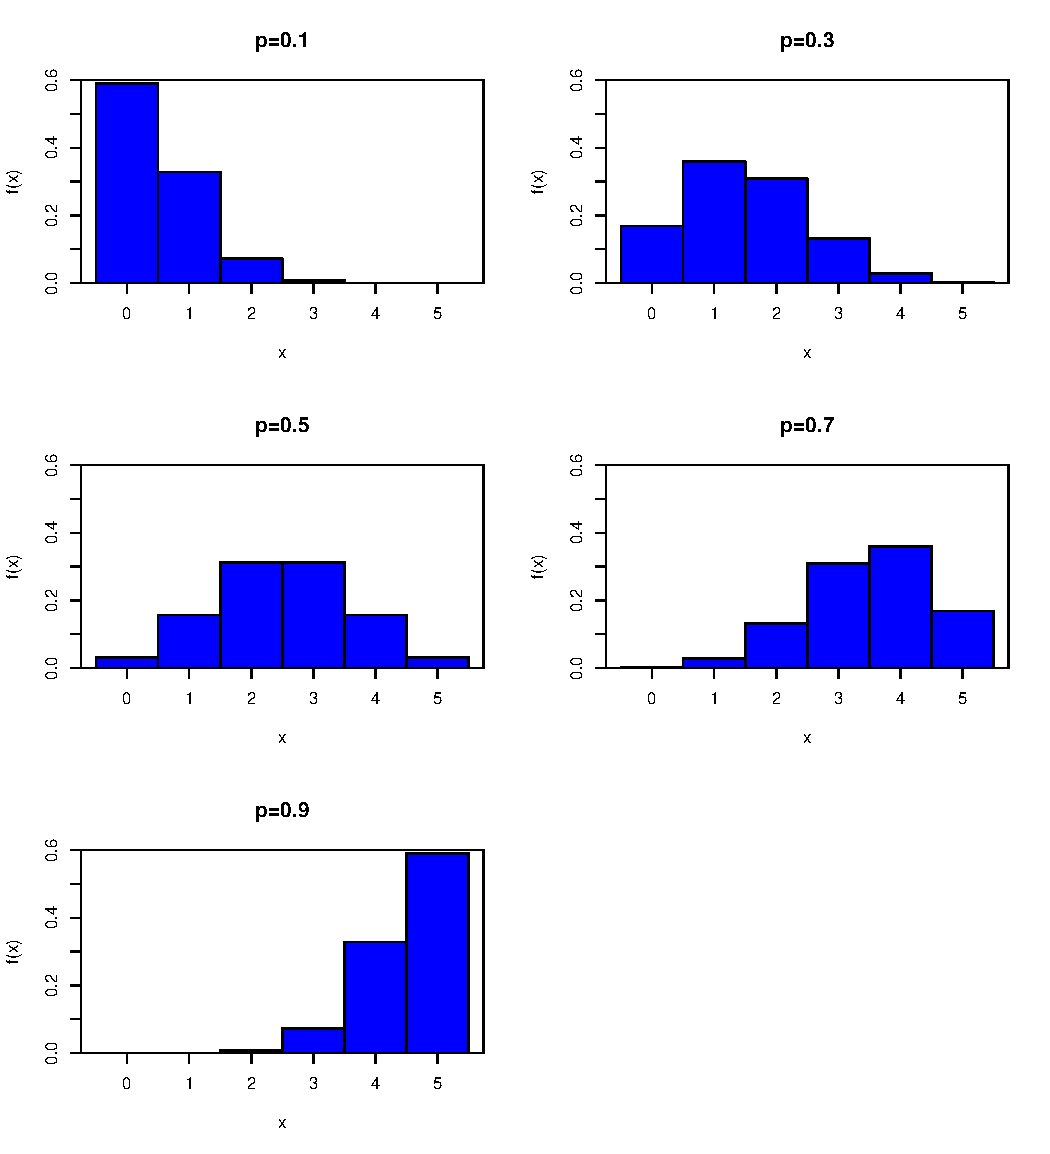
\includegraphics[width=0.8\textwidth]{figure/unnamed-chunk-3-1} 

}



\end{knitrout}




}

\clearpage
\item P. 322: 1

{\color{red} Use equation (5-3) with $n = 6$ and $p = 0.9$.}
\begin{enumerate}

\item (3 points)

$P(X = 6) = 0.531$
\item (3 points)

$P(X \ge 4) = 0.984$

\item (3 points)

$P(X < 4) = 1 - P(X \ge 4) = 0.016$

\item (3 points)

$E(X) = np = 5.4$

\item (3 points)

$Var(X) = np(1 - p) = 0.54,\, SD(X) = \sqrt{0.54} = 0.735$
\end{enumerate}


\item P. 322: 2

{\color{red} Use equation (5-3) with $n = 10$ and $p = 0.15$.}
\begin{enumerate}
\item (3 points)

$P(X = 2) = 0.276$

\item (3 points)

$P(X \ge 1) = 1 - P(X < 1) = 1 - P(X = 0) = 1 - 0.197 = 0.803$

\item (3 points)

$E(X) = np = 1.5$

\item (3 points)

$Var(X) = np(1 - p) = 1.275$

\item (3 points)

$SD(X) = \sqrt{1.275} = 1.129$

Use equation (5-3) with $n = 6$ and $p = 0.9$.
\end{enumerate}


\end{enumerate}
%\newpage 
%\nocite{*}
%\bibliographystyle{plainnat} 
%\bibliography{}
\end{document}
